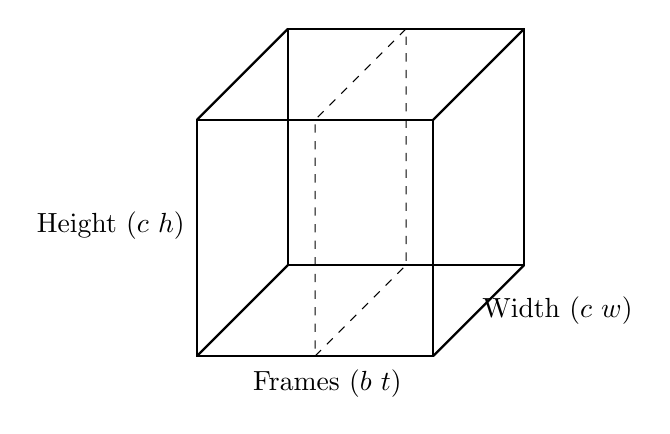
\begin{tikzpicture}
    % Cube points
    \coordinate (A) at (0, 0, 0);
    \coordinate (B) at (3, 0, 0);
    \coordinate (C) at (3, 3, 0);
    \coordinate (D) at (0, 3, 0);
    \coordinate (E) at (0, 0, 3);
    \coordinate (F) at (3, 0, 3);
    \coordinate (G) at (3, 3, 3);
    \coordinate (H) at (0, 3, 3);

    % Draw cube
    \draw[thick] (A) -- (B) -- (C) -- (D) -- cycle;
    \draw[thick] (E) -- (F) -- (G) -- (H) -- cycle;
    \draw[thick] (A) -- (E);
    \draw[thick] (B) -- (F);
    \draw[thick] (C) -- (G);
    \draw[thick] (D) -- (H);

    % Draw slice in middle
    \draw[dashed] (1.5, 0, 3) -- (1.5, 0, 0) -- (1.5, 3, 0) -- (1.5, 3, 3) -- cycle;
    
    % Axes
    \node at (0.5, -1.5, 0) {Frames $(b\ t)$}; 
    \node at (-2.25, 0.5, 0) {Height $(c\ h)$};
    \node at (4.0, 0, 1.5) {Width $(c\ w)$};

    % Add slice label
    % \node at (1.5, 3.5) {$(b\ t)\ c$};
\end{tikzpicture}